\documentclass{scrartcl}
\usepackage[utf8]{inputenc}
\PassOptionsToPackage{hyphens}{url}
\usepackage{hyperref}
\usepackage{url}
\usepackage{natbib}
\usepackage{graphicx}
\usepackage{amsmath}
\usepackage{xcolor}
\usepackage{booktabs}
\usepackage{tabularx}
\newcolumntype{Y}{>{\raggedright\arraybackslash}X}
\usepackage{listings}
\usepackage{enumitem}
\setlist{itemsep=1pt, parsep=0pt, topsep=3pt}
\usepackage{tikz}
\usetikzlibrary{arrows.meta, positioning, fit, calc, shapes.multipart}
\usepackage{pgfplots}
\pgfplotsset{compat=1.18}
\usepgfplotslibrary{groupplots}

% Chart palette: two categorical slots validated for colour-blind
% separation on a light surface, plus text and chrome greys.
\definecolor{series1}{HTML}{2A78D6}
\definecolor{series2}{HTML}{EB6834}
\definecolor{textprimary}{HTML}{0B0B0B}
\definecolor{textsecondary}{HTML}{52514E}
\definecolor{gridline}{HTML}{E4E3DF}
\definecolor{axisline}{HTML}{8A8983}
\pgfplotsset{
  thunkplot/.style={
    axis lines*=left,
    axis line style={axisline, line width=0.4pt},
    tick style={axisline, line width=0.4pt},
    major grid style={gridline, line width=0.4pt},
    tick label style={font=\scriptsize, text=textsecondary},
    label style={font=\scriptsize, text=textsecondary},
    title style={font=\small, text=textprimary},
    legend style={font=\scriptsize, draw=none, fill=white, fill opacity=0.9, text opacity=1},
    legend cell align=left,
    scaled ticks=false,
  },
  thunkhbar/.style={
    xbar, bar width=8pt, xmajorgrids,
    every axis plot post/.append style={draw=none},
    nodes near coords,
    nodes near coords align={horizontal},
    every node near coord/.append style={font=\scriptsize, text=textprimary, anchor=west, inner sep=2pt},
    point meta=explicit symbolic,
    y tick label style={font=\scriptsize, text=textprimary},
  },
  thunkline/.style={line width=1pt, mark=*, mark size=1.8pt},
}
\tikzset{refline/.style={textsecondary, line width=0.4pt}}
% Sequence diagram and worker state machine: Mermaid renderings (figures/*.mmd)
% or the TikZ originals (figures/tikz-*.tex). Flip the switch to compare.
% Regenerate the Mermaid PDFs from figures/ with:
%   mmdc -i mermaid-steal.mmd -o mermaid-steal.pdf --pdfFit -c mermaid-config.json -p puppeteer-config.json -b white
%   mmdc -i mermaid-worker.mmd -o mermaid-worker.pdf --pdfFit -c mermaid-config.json -p puppeteer-config.json -b white
\newif\ifmermaid \mermaidtrue
% Let tall figures share a page with text instead of each taking a page.
\renewcommand{\topfraction}{0.9}
\renewcommand{\bottomfraction}{0.8}
\renewcommand{\textfraction}{0.07}
\renewcommand{\floatpagefraction}{0.8}
\usepackage{cleveref} % this must be the last package to be loaded

\newcommand{\emailaddr}[1]{\href{mailto:#1}{\texttt{#1}}}

\lstset{
  basicstyle=\ttfamily\footnotesize,
  columns=fullflexible,
  keepspaces=true,
  frame=single,
  framerule=0.3pt,
  xleftmargin=2mm,
  xrightmargin=2mm,
  breaklines=true,
  showstringspaces=false,
  aboveskip=6pt,
  belowskip=6pt
}
\addtokomafont{caption}{\small}

\title{\LARGE Thunk}
\subtitle{A Peer-to-Peer Evaluator for Pure Functional Computations\\
Final Report for the Distributed Systems Course, academic year 2025/2026}

\author{
    Yosberto Baro Carbonell \\ \emailaddr{yosberto.baro@studio.unibo.it}
}

\date{\today}

\begin{document}

\maketitle

\begin{abstract}
Thunk is a distributed runtime that evaluates pure functional computations on a cluster of peer nodes, without a central coordinator.
%
Computations are expressed in a small functional language whose only parallel construct is a divide-and-conquer primitive, map and reduce are then built on it.
%
Programs travel between nodes as data, so a node needs no prior knowledge of the programs it helps to run.
%
Work is distributed by randomized work stealing and, since computations are pure, a piece lost with a failed node is simply recomputed by the node waiting for it: crashes are tolerated without replication.
%
It was validated with automated tests on real additional nodes and with experiments on one machine and on two machines connected over the Internet.
\end{abstract}

% Disclaimer (if needed). The course template asks to declare any tool or
% service used during the preparation of the work. To be decided and written
% by the author; uncomment and complete, or delete.
%
% \section*{Disclaimer}
%
% During the preparation of this work, the author used [NAME TOOL / SERVICE] to [REASON].
% After using this tool/service, the author reviewed and edited the content as needed
% and takes full responsibility for the content of the final report/artifact.

\section{Concept}\label{concept}

\subsection{Product Description}

This project implements a \emph{distributed evaluator for pure functional computations} in the form of a library and a set of cooperating nodes.
%
The system is used programmatically, by submitting a program and an input value on any node of the cluster, and it is observed through its command-line output and logs.

The primary use case is the execution of computations that are naturally recursive and data-parallel, such as sorting, counting or rendering, on a small group of machines where:
%
\begin{itemize}
  \item no machine should play a special role;
  \item machines may fail while a computation is running;
  \item the computation is not known in advance by the machines that will help run it.
\end{itemize}

Users write a program in the Thunk language, start a job from a shell on one of the nodes, and wait for its result.
%
Interaction is occasional: a job runs for seconds or minutes and returns a single value.
%
There is no hierarchy, every node is equally able to submit jobs, compute pieces of them, and help other nodes.
%
No persistent data is stored: a program, its input and all intermediate results exist in memory only for the duration of the job.

The system follows a \emph{fork-join} model with \emph{randomized work stealing}: a node that splits a problem keeps one half and exposes the other, and idle nodes take exposed work from randomly chosen peers.
%
Since the language is pure, the result never depends on where or when each piece was computed, and a piece lost with a failed node can simply be computed again.

\subsection{Why Distribution Is Needed}

\begin{itemize}
  \item \textbf{Computation speed-up:} a divide-and-conquer computation can be split into many independent pieces, and the processors of several machines can work on them at the same time.

  \item \textbf{Resource sharing:} idle machines contribute their processing time to jobs submitted elsewhere, without having to know the program in advance.

  \item \textbf{Fault tolerance:} a centralized scheduler would be a single point of failure; without one, the loss of a machine only loses the work it was doing.

  \item \textbf{Educational value:} a practical study of scheduling without a coordinator, of moving computations as data between machines, of failure detection between remote processes, and of the relation between purity and fault tolerance.
\end{itemize}

\section{Requirements Elicitation and Analysis}\label{requirements}

\subsection{Glossary}

\begin{itemize}
  \item \textbf{Program:} a sequence of top-level definitions written in the Thunk language. Running a program means applying its definition called \texttt{main} to an input value.
  \item \textbf{Prelude:} the standard library of the language, itself written in the language and available on every node.
  \item \textbf{Job:} one execution of a program on an input, submitted on a node called its \emph{origin}.
  \item \textbf{Divide and conquer (\texttt{dc}):} the only parallel construct of the language (\cref{modelling}).
  \item \textbf{Piece:} a part of a job waiting to be computed: a value together with the functions that say how to split it, solve it and combine the results.
  \item \textbf{Owner:} the process that split a piece off and is waiting for its result.
  \item \textbf{Thief:} a node that takes a piece from another node.
  \item \textbf{Threshold:} the criterion that decides when a value is small enough to be solved directly. In Thunk it is a predicate written by the user.
\end{itemize}

\subsection{Functional Requirements}

Each requirement is followed by its acceptance criterion.
%
\begin{itemize}
  \item \textbf{FR1, Functional Language:} users must be able to express computations as programs in a pure functional language offering map, reduce and a divide-and-conquer primitive.
  \emph{Acceptance:} the library functions and the demonstration programs return the same results as equivalent native implementations.

  \item \textbf{FR2, Recursive Decomposition:} a divide-and-conquer computation must be split recursively until the user's threshold states that a part is small enough; the parts must then be solved and their results combined in order.
  \emph{Acceptance:} splitting stops exactly where the threshold says, results are combined in the order of the split, and misuse (a threshold that does not return a boolean, a split that does not produce two parts) is reported as an error.

  \item \textbf{FR3, Decentralized Work Stealing:} any node must be able to submit a job; pieces of the job must be taken and computed by other nodes, and their results combined into the result of the job.
  \emph{Acceptance:} a job submitted on a node that is not allowed to compute pieces itself returns the correct result, and the other nodes report stolen pieces.

  \item \textbf{FR4, Program Distribution:} a program must only have to be known by the node that submits it; the other nodes must obtain it when they first need it.
  \emph{Acceptance:} a job whose program uses definitions that exist only on the submitting node completes correctly on the cluster.

  \item \textbf{FR5, Error Reporting:} an error in the program, wherever it occurs, must be reported to the submitter as the same error a sequential execution would have produced.
  \emph{Acceptance:} a program that fails in a piece computed by a remote node raises the same error at the submitter.

  \item \textbf{FR6, Recovery from Node Failures:} a job must complete with the correct result if a node that holds pieces of it crashes or disconnects while it runs.
  \emph{Acceptance:} after intentionally stopping a node during a job, the job returns the same result it returns without the failure.

  \item \textbf{FR7, Demonstration Workloads:} word count and mergesort must be runnable from the command line on one node or on the cluster, with a check of the result.
  \emph{Acceptance:} every run of the demonstrations reports a correct result under every scheduling mode.

  \item \textbf{FR8, Dynamic Membership (extension):} a node must be able to join a running cluster knowing a single existing node, and nodes that leave must be forgotten, without any central register.
  \emph{Acceptance:} a node started with one seed ends up connected to every node of the cluster, and a node that joins while a job runs takes part in that job.
\end{itemize}

\subsection{Non-Functional Requirements}

\begin{itemize}
  \item \textbf{Determinism:} the result of a job must not depend on which node computed which piece, on the number of nodes, or on the order in which pieces finish.
  \item \textbf{Decentralization:} no node may have a special role in scheduling.
  \item \textbf{Liveness under failure:} a job must never wait forever because a remote participant failed.
  \item \textbf{Low distribution overhead:} on the same hardware, running a job across nodes must cost little compared with running it on local processes only.
  \item \textbf{Configurability:} the peers of a node and the amount of work it performs locally must be configurable through environment variables.
  \item \textbf{Observability:} each node must expose counters of stolen, given, evaluated and recovered pieces, and the state of the whole cluster must be observable live while a job runs.
\end{itemize}

\subsection{Implementation Requirements}

The system is implemented in Elixir on the Erlang virtual machine (BEAM), as agreed in the project proposal: the platform provides lightweight processes, message passing between machines and failure notification between remote processes.
%
Nodes communicate through the native distribution of the Erlang runtime, without external middleware, and Docker Compose runs a multi-node cluster reproducibly.
%
No third-party libraries are used, so that every distributed mechanism is implemented and studied directly.

\subsection{Relevant Distributed System Features}
\label{ds-features}

\begin{itemize}
  \item \textbf{Transparency:} location transparency is central. A program cannot observe where its pieces run, and the same program runs unchanged on one process, on several local processes or on several nodes. Failure transparency is provided for node crashes, which are hidden by recomputation, but intentionally not for errors in the program, which are reported.

  \item \textbf{Fault Tolerance and Dependability:} the system tolerates crash failures of the nodes that help compute a job, not of the node that submitted it. It holds no data that could be lost, only computation, which purity makes repeatable (\cref{fault-tolerance}).

  \item \textbf{Scalability:} the system targets a handful of machines on a local network. Work stealing only requires each node to know its peers, and the amount of coordination grows with the number of stolen pieces, not with the size of the input.

  \item \textbf{Consistency:} there is no replicated state; the only shared data, the definitions of a job, are immutable, and consistency of the results follows from purity (\cref{data-and-consistency-issues}).

  \item \textbf{Resource Sharing:} the shared resource is processor time. Idle nodes pull work from busy ones.

  \item \textbf{Maintainability and Evolvability:} the language has only thirteen primitive operations; everything else, including map, reduce and sorting, is library code written in the language itself, so the library can grow without changing the runtime.

  \item \textbf{Performance and Efficiency:} the relevant metrics are the time to complete a job, the overhead of distribution compared with local execution, and the amount of data carried by each piece of work, since pieces may cross the network.

  \item \textbf{Not goals:} security, since the system assumes a trusted private network (\cref{security}); openness, since all nodes run the same software and speak the native protocol of the runtime; and cost, since the system runs on machines the user already has and uses no paid service.
\end{itemize}

\section{Design}\label{design}

\subsection{Architecture}\label{architecture}

The system adopts a fully decentralized \emph{peer-to-peer} architecture.
%
Every node is architecturally identical: it can accept a job, split work, compute pieces and give pieces to others.
%
There is no master, no central queue and no shared database.

Within a job, computation follows the \emph{fork-join} model with \emph{randomized work stealing} introduced by the Cilk runtime~\cite{frigo1998cilk} and analysed by Blumofe and Leiserson~\cite{blumofe1999scheduling}.
%
A process that splits a problem keeps one half to work on and exposes the other in a deque; nodes with nothing to do steal from the deques of other nodes, choosing the victim at random.
%
This choice is motivated by:
%
\begin{itemize}
  \item \textbf{No single point of failure:} a master that assigns tasks, as in MapReduce-like systems~\cite{dean2004mapreduce}, would be a component every job depends on.
  \item \textbf{No global knowledge:} random stealing only requires each node to know its peers, and it is known to balance load efficiently with few steal attempts~\cite{blumofe1999scheduling}.
  \item \textbf{Local bookkeeping:} whoever splits a piece waits for its result. No component keeps a table of the pending tasks of a job, and the end of a job is simply the return of its first computation (\cref{behaviour}).
\end{itemize}

Two alternatives were discarded.
%
An \emph{explicit task tree}, in which the submitting node records every piece and receives completion notices, gives cleaner accounting but turns that node into a bookkeeper for the whole job, close to a coordinator.
%
A \emph{shared store}, such as a message queue holding pieces and results, would route all communication through a central component, give every piece an identity and every result an address, and make serialization a concern of the application.

\begin{figure}
  \centering
  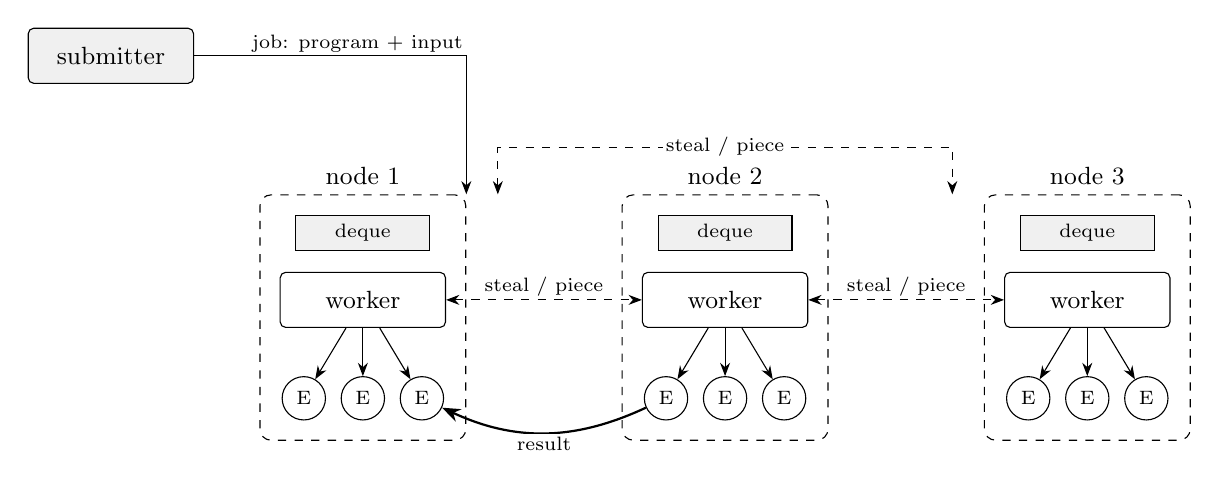
\begin{tikzpicture}[
      >=Stealth,
      wk/.style={draw, rounded corners=2pt, minimum width=21mm, minimum height=7mm, font=\small},
      dq/.style={draw, minimum width=17mm, minimum height=4.5mm, font=\scriptsize, fill=black!6},
      ev/.style={draw, circle, minimum size=5.5mm, inner sep=0pt, font=\scriptsize},
      grp/.style={draw, dashed, rounded corners=4pt, inner sep=2.5mm},
      lbl/.style={font=\scriptsize, fill=white, inner sep=1pt}]
    \foreach \i/\x in {1/0, 2/4.6, 3/9.2} {
      \node[dq] (q\i) at (\x, 0.85) {deque};
      \node[wk] (w\i) at (\x, 0) {worker};
      \node[ev] (ea\i) at (\x-0.75, -1.25) {E};
      \node[ev] (eb\i) at (\x, -1.25) {E};
      \node[ev] (ec\i) at (\x+0.75, -1.25) {E};
      \draw[->] (w\i) -- (ea\i);
      \draw[->] (w\i) -- (eb\i);
      \draw[->] (w\i) -- (ec\i);
      \node[grp, fit=(q\i)(w\i)(ea\i)(ec\i), label={[font=\small]above:node \i}] (n\i) {};
    }
    \node[wk, fill=black!6] (sub) at (-3.2, 3.1) {submitter};
    \draw[->] (sub.east) -| node[lbl, above, pos=0.3] {job: program + input} (n1.north east);
    \draw[<->, dashed] (w1) -- node[lbl, above] {steal / piece} (w2);
    \draw[<->, dashed] (w2) -- node[lbl, above] {steal / piece} (w3);
    \draw[<->, dashed] ([xshift=4mm]n1.north east) -- ++(0,0.6) -| node[lbl, pos=0.25] {steal / piece} ([xshift=-4mm]n3.north west);
    \draw[->, thick] (ea2) to[bend left=25] node[lbl, below] {result} (ec1);
  \end{tikzpicture}
  \caption{Decentralized architecture of a Thunk cluster. Every node has the same structure: a worker holding a deque of pieces, and evaluator processes (E) that compute pieces. Workers exchange steal requests and pieces; the result of a stolen piece is sent directly to the process waiting for it.}
  \label{fig:architecture}
\end{figure}

\subsection{Infrastructure}\label{infrastructure}

The system is composed exclusively of \emph{homogeneous nodes}, each an instance of the Erlang virtual machine running the Thunk application (\cref{fig:architecture}).
%
Each node includes four logical components:
%
\begin{enumerate}
  \item \textbf{Worker:} a long-lived process that holds the node's deque of stealable pieces and a cache of the programs of the jobs it has met, and decides when to steal.
  \item \textbf{Evaluators:} short-lived processes, each computing one piece by interpreting the program.
  \item \textbf{Evaluator supervisor:} starts evaluators and isolates their failures, so that a failing program cannot bring the worker down.
  \item \textbf{Membership process:} keeps the list of the other nodes and connects to the ones it learns about (\cref{behaviour}).
\end{enumerate}

A client is not a separate component: submitting a job means calling the library on any node, which then acts as the origin of the job.
%
In the demonstrations, the submitting node is an additional short-lived node started next to the others.

Nodes are meant to run on different machines of a local network; in the Docker Compose deployment they run as containers on a shared virtual network.
%
Each node is identified by a name of the form \texttt{name@host}.
%
A node is started with a list of \emph{seeds}, names of existing nodes passed through an environment variable, and needs only one of them to be reachable; it then discovers the rest of the cluster by gossip.
%
The Erlang name service on each host maps node names to ports, and in Docker Compose host names are resolved by the container DNS.

\subsection{Modelling}\label{modelling}

\paragraph{The language.}
The language is pure, strict, lexically scoped and dynamically typed.
%
Its values are integers of arbitrary size, booleans, strings, lists and functions.
%
A program is a sequence of definitions, and everything in it is an expression: \texttt{fn} builds a function, \texttt{let x = e in body} binds one name, \texttt{if c then a else b} chooses a branch, and \texttt{f(x, y)} is a call.
%
There are thirteen primitive operations: arithmetic and comparison on integers, construction and inspection of lists, and conversion between strings and lists of character codes; the infix operators \texttt{+ - * / \% < == ::} are only a notation for them.
%
Everything else, from list functions to sorting and the parallel operations, is written in the language itself, in the prelude.
\begin{lstlisting}
def isqrt_iter(n, x) =
  let y = (x + n / x) / 2 in
  if y < x then isqrt_iter(n, y) else x
\end{lstlisting}
%
The parser is generated from a grammar, in the tradition of Yacc~\cite{johnson1975yacc}, and turns a program into nested lists, the representation of programs in Lisp~\cite{mccarthy1960recursive}: the definition above becomes a list headed by \texttt{def}, its body a list headed by \texttt{let}, and each operator a call of its primitive.
%
The interpreter and the runtime only ever see these lists, and so do the pieces of work that travel between nodes.

The only parallel construct is
\begin{center}
\texttt{dc(\emph{value}, \emph{small?}, \emph{split}, \emph{base}, \emph{merge})}
\end{center}
whose meaning is
\[
\mathit{solve}(v) =
\begin{cases}
\mathit{base}(v) & \text{if } \mathit{small?}(v)\\
\mathit{merge}(\mathit{solve}(l), \mathit{solve}(r)) & \text{otherwise, where } [l, r] = \mathit{split}(v)
\end{cases}
\]
%
The threshold is part of the user's predicate, so the runtime needs no notion of size.
%
The merge always receives the left result first, so the result does not depend on where each half was computed or which one finished first.
%
Parallel map and reduce are ordinary definitions:
\begin{lstlisting}
def pmap(f, xs, small?) = dc(xs, small?, halves, pmap_base(f), append)

def reduce(op, xs, small?) = dc(xs, small?, halves, reduce_base(op), op)

def mergesort(xs, small?) = dc(xs, small?, halves, insertion_sort, merge_sorted)
\end{lstlisting}
%
Parallelism is therefore never inferred by the runtime: choosing \texttt{reduce} instead of the sequential \texttt{fold} is how a user states that an operation is associative and may be computed in parallel.

\paragraph{Domain entities.}
A \emph{program} is a table of named definitions, obtained by parsing the source and evaluating each definition; a \emph{job} is identified by a unique reference and by its origin node, which keeps the program.
%
A \emph{work} is a value together with the four functions of the \texttt{dc} that produced it; functions are closures, that is, data: the parameter names, the body and the captured variables.
%
A \emph{piece} is a work together with a unique reference, the address of the process waiting for its result, and the identity of its job.
%
All entities are held in memory by the nodes that use them (\cref{fig:classes}).
%
A piece lives in exactly one place at a time: in the deque of the node that created it, in the hands of the evaluator computing it, or nowhere once solved.

\begin{figure}
  \centering
  \resizebox{\linewidth}{!}{%
  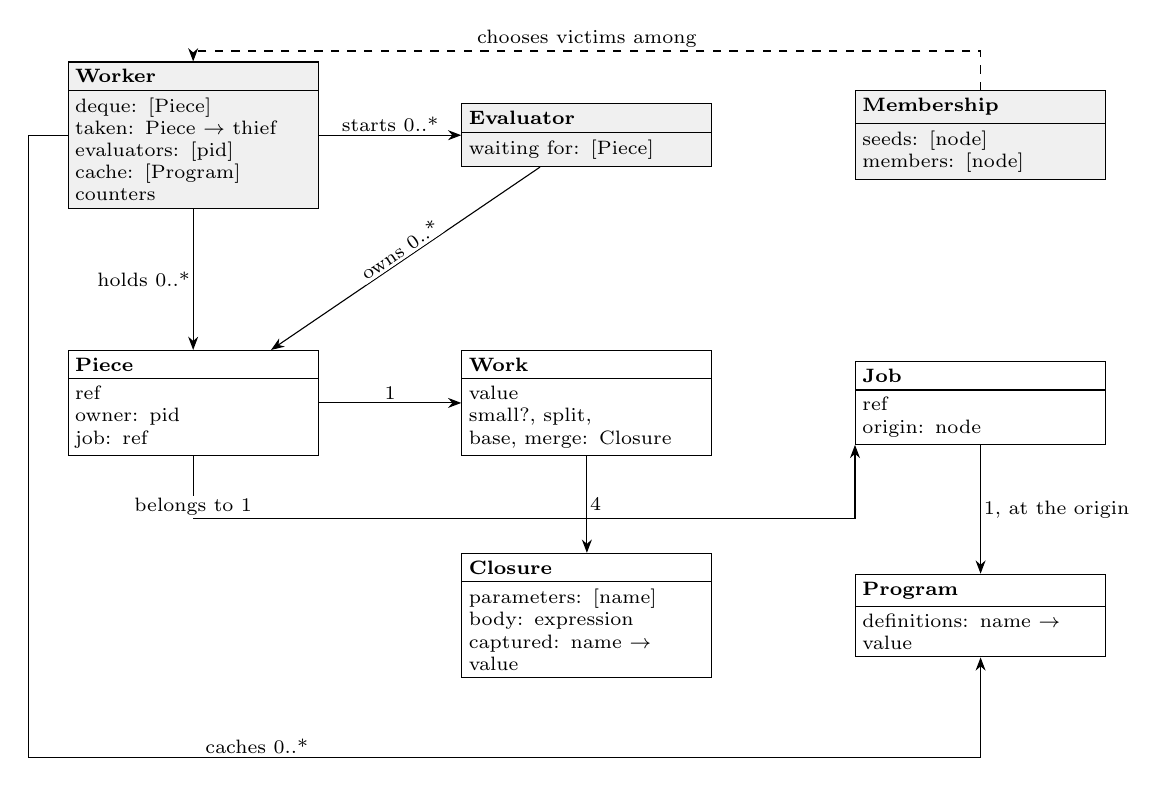
\begin{tikzpicture}[
      >=Stealth, font=\scriptsize,
      cls/.style={draw, rectangle split, rectangle split parts=2,
        rectangle split part align={center, left}, text width=30mm,
        inner sep=2.5pt, align=left},
      comp/.style={cls, fill=black!6},
      rel/.style={->, font=\scriptsize},
      lbl/.style={font=\scriptsize, fill=white, inner sep=1pt}]
    \node[comp] (worker) at (0,0) {\textbf{Worker}\nodepart{second}deque: [Piece]\\taken: Piece $\to$ thief\\evaluators: [pid]\\cache: [Program]\\counters};
    \node[comp] (eval) at (5,0) {\textbf{Evaluator}\nodepart{second}waiting for: [Piece]};
    \node[comp] (memb) at (10,0) {\textbf{Membership}\nodepart{second}seeds: [node]\\members: [node]};
    \node[cls] (piece) at (0,-3.4) {\textbf{Piece}\nodepart{second}ref\\owner: pid\\job: ref};
    \node[cls] (work) at (5,-3.4) {\textbf{Work}\nodepart{second}value\\small?, split,\\base, merge: Closure};
    \node[cls] (job) at (10,-3.4) {\textbf{Job}\nodepart{second}ref\\origin: node};
    \node[cls] (closure) at (5,-6.1) {\textbf{Closure}\nodepart{second}parameters: [name]\\body: expression\\captured: name $\to$ value};
    \node[cls] (program) at (10,-6.1) {\textbf{Program}\nodepart{second}definitions: name $\to$ value};
    \draw[rel] (worker) -- node[lbl, left] {holds 0..*} (piece);
    \draw[rel] (worker) -- node[lbl, above] {starts 0..*} (eval);
    \draw[rel] (eval) -- node[lbl, above, sloped] {owns 0..*} (piece);
    \draw[rel] (piece) -- node[lbl, above] {1} (work);
    \draw[rel] (work) -- node[lbl, right] {4} (closure);
    \draw[rel] (piece.south) |- node[lbl, pos=0.75, above] {belongs to 1} ([yshift=-8mm]piece.south) -| (job.south west);
    \draw[rel] (job) -- node[lbl, right] {1, at the origin} (program);
    \draw[rel] (worker.west) -- ++(-0.5,0) |- node[lbl, pos=0.62, above] {caches 0..*} (program.south |- 0,-7.9) -- (program.south);
    \draw[rel, dashed] (memb.north) -- ++(0,0.5) -| node[lbl, pos=0.25, above] {chooses victims among} (worker.north);
  \end{tikzpicture}}
  \caption{Domain entities and the components that hold them. Grey boxes are processes, white boxes are immutable data. A piece points to its work and to the evaluator waiting for it; the four functions of a work are closures, so a piece carries whatever they captured.}
  \label{fig:classes}
\end{figure}

\paragraph{Domain events.}
Job Submitted; Piece Pushed (a right half becomes available); Piece Stolen, or Taken Back by its owner; Piece Claimed (a thief started computing it); Result Returned; Piece Lost (its evaluator or node failed); Program Fetched (a node obtains the definitions of a job).

\paragraph{Messages.}
\Cref{tab:messages} lists the messages exchanged between processes.
%
Apart from fetching a program, which is a request followed by a reply, all messages are asynchronous.

\begin{table}
  \centering
  \small
  \begin{tabularx}{\textwidth}{@{}lllY@{}}
    \toprule
    Message & From & To & Meaning \\
    \midrule
    push & evaluator & local worker & a right half is available \\
    take back & evaluator & local worker & the owner wants its piece back; the reply is the piece, or the worker that took it \\
    steal & worker & remote worker & request for the oldest piece \\
    piece / none & worker & thief & reply to a steal request \\
    claimed & thief worker & owner & the piece is being computed by a given evaluator \\
    result & evaluator & owner & the value of a stolen piece \\
    failed & thief worker & owner & the evaluator of a piece died, with the reason \\
    get job & evaluator & origin worker & request for the program of a job \\
    pull & membership & random peer & request for the peer's list of members \\
    push & membership & asking node & the list of members, to connect to the unknown ones \\
    \bottomrule
  \end{tabularx}
  \caption{Messages exchanged between Thunk processes.}
  \label{tab:messages}
\end{table}

\paragraph{State.}
The state of a node is the state of its worker (\cref{fig:classes}); the state of a job in progress is spread over the evaluators computing it, each remembering the pieces it has split off and is waiting for.
%
There is no global state.

\subsection{Interaction}\label{interaction}

Nodes interact through the steal protocol shown in \cref{fig:steal}:
%
\begin{enumerate}
  \item An evaluator that splits a value pushes the right half to its node's worker and continues with the left half.
  \item A worker with spare capacity and an empty deque sends a steal request to a peer chosen at random.
  \item The victim answers with its oldest piece, or with \emph{none}.
  \item The thief's worker starts an evaluator for the piece and tells the owner which process is computing it.
  \item When the owner has finished its own half, it asks its worker for the right half back. If nobody took it, the owner computes it itself; otherwise it waits for the result.
  \item The thief's evaluator sends the result directly to the owner, which combines it with its own.
\end{enumerate}

The victim gives away its \emph{oldest} piece, while a node's own evaluators take the \emph{newest}.
%
In a divide-and-conquer tree the oldest piece is the largest: one network round trip transfers the most work, and the thief can split it further and become self-sufficient.
%
The newest piece is the smallest, and its data is already local.
%
\Cref{fig:deque} shows why on a list of sixteen elements.

\begin{figure}[tbp]
  \centering
  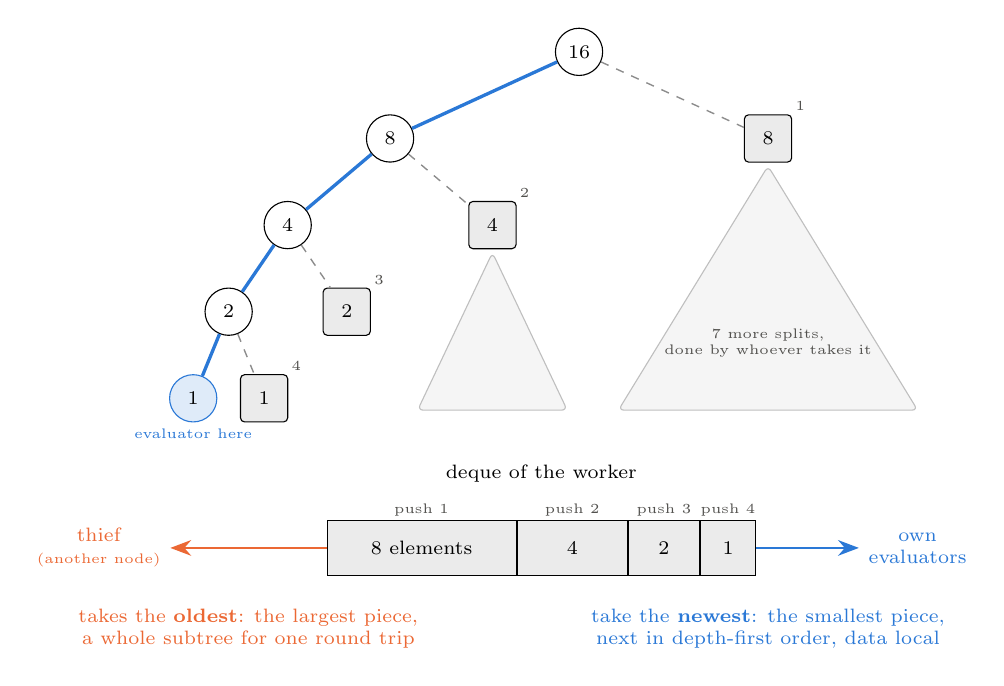
\begin{tikzpicture}[
    >=Stealth,
    ev/.style={draw, circle, minimum size=6mm, inner sep=0pt, font=\scriptsize},
    pc/.style={draw, rounded corners=1.5pt, minimum size=6mm, inner sep=0pt, font=\scriptsize, fill=black!8},
    tag/.style={font=\tiny, text=textsecondary, inner sep=1pt},
    lbl/.style={font=\scriptsize, fill=white, inner sep=1pt},
    path/.style={series1, line width=1.2pt},
    push/.style={black!45, line width=0.5pt, dashed},
    sub/.style={fill=black!4, draw=black!25, line width=0.4pt, rounded corners=2pt},
    cell/.style={draw, fill=black!8, minimum height=7mm, inner sep=0pt, font=\scriptsize}]

  % Subtrees still inside the two largest pushed pieces.
  \fill[sub] (2.4,-1.45) -- (0.5,-4.55) -- (4.3,-4.55) -- cycle;
  \node[tag, align=center] at (2.4,-3.7) {7 more splits,\\done by whoever takes it};
  \fill[sub] (-1.1,-2.55) -- (-2.05,-4.55) -- (-0.15,-4.55) -- cycle;

  % The evaluator's own path, always the left half.
  \node[ev] (r) at (0,0) {16};
  \node[ev] (a1) at (-2.4,-1.1) {8};
  \node[ev] (a2) at (-3.7,-2.2) {4};
  \node[ev] (a3) at (-4.45,-3.3) {2};
  \node[ev, fill=series1!15, draw=series1] (a4) at (-4.9,-4.4) {1};
  \draw[path] (r) -- (a1);
  \draw[path] (a1) -- (a2);
  \draw[path] (a2) -- (a3);
  \draw[path] (a3) -- (a4);
  \node[tag, below=1pt of a4, text=series1] {evaluator here};

  % The right halves, pushed to the deque on the way down.
  \node[pc] (p1) at (2.4,-1.1) {8};
  \node[pc] (p2) at (-1.1,-2.2) {4};
  \node[pc] (p3) at (-2.95,-3.3) {2};
  \node[pc] (p4) at (-4.0,-4.4) {1};
  \draw[push] (r) -- (p1);
  \draw[push] (a1) -- (p2);
  \draw[push] (a2) -- (p3);
  \draw[push] (a3) -- (p4);
  \foreach \p/\n in {p1/1, p2/2, p3/3, p4/4}
    \node[tag, anchor=south west] at (\p.north east) {\n};

  % The deque, in push order: oldest on the left, newest on the right.
  \node[cell, minimum width=24mm] (d1) at (-2.0,-6.3) {8 elements};
  \node[cell, minimum width=14mm, right=0pt of d1] (d2) {4};
  \node[cell, minimum width=9mm, right=0pt of d2] (d3) {2};
  \node[cell, minimum width=7mm, right=0pt of d3] (d4) {1};
  \foreach \d/\n in {d1/1, d2/2, d3/3, d4/4}
    \node[tag, anchor=south] at (\d.north) {push \n};
  \node[font=\scriptsize, anchor=south] at ([yshift=3.5mm]$(d1.north west)!0.5!(d4.north east)$) {deque of the worker};

  \node[font=\scriptsize, align=center, text=series2] (thief) at (-6.1,-6.3) {thief\\\tiny(another node)};
  \node[font=\scriptsize, align=center, text=series1] (own) at (4.3,-6.3) {own\\evaluators};
  \draw[->, series2, line width=1pt] (d1.west) -- (thief.east);
  \draw[->, series1, line width=1pt] (d4.east) -- (own.west);

  \node[font=\scriptsize, align=center, anchor=north, text=series2] at (-4.2,-6.95)
    {takes the \textbf{oldest}: the largest piece,\\a whole subtree for one round trip};
  \node[font=\scriptsize, align=center, anchor=north, text=series1] at (2.4,-6.95)
    {take the \textbf{newest}: the smallest piece,\\next in depth-first order, data local};
\end{tikzpicture}

  \caption{The two ends of the deque. Numbers are sizes in elements. An evaluator descends along the left half at every level and pushes the right half, so the deque holds pieces of decreasing size in push order. A thief takes the oldest piece, a whole subtree that it splits further on its own node; the node's own evaluators take the newest, which is the next leaf in depth-first order.}
  \label{fig:deque}
\end{figure}

From a communication perspective, a stolen piece costs a request, a reply, a claim and a result: four messages, independently of the size of the job.
%
The amount of data they carry, however, depends on what the piece contains, which is discussed in \cref{data-and-consistency-issues}.

\begin{figure}
  \centering
  \ifmermaid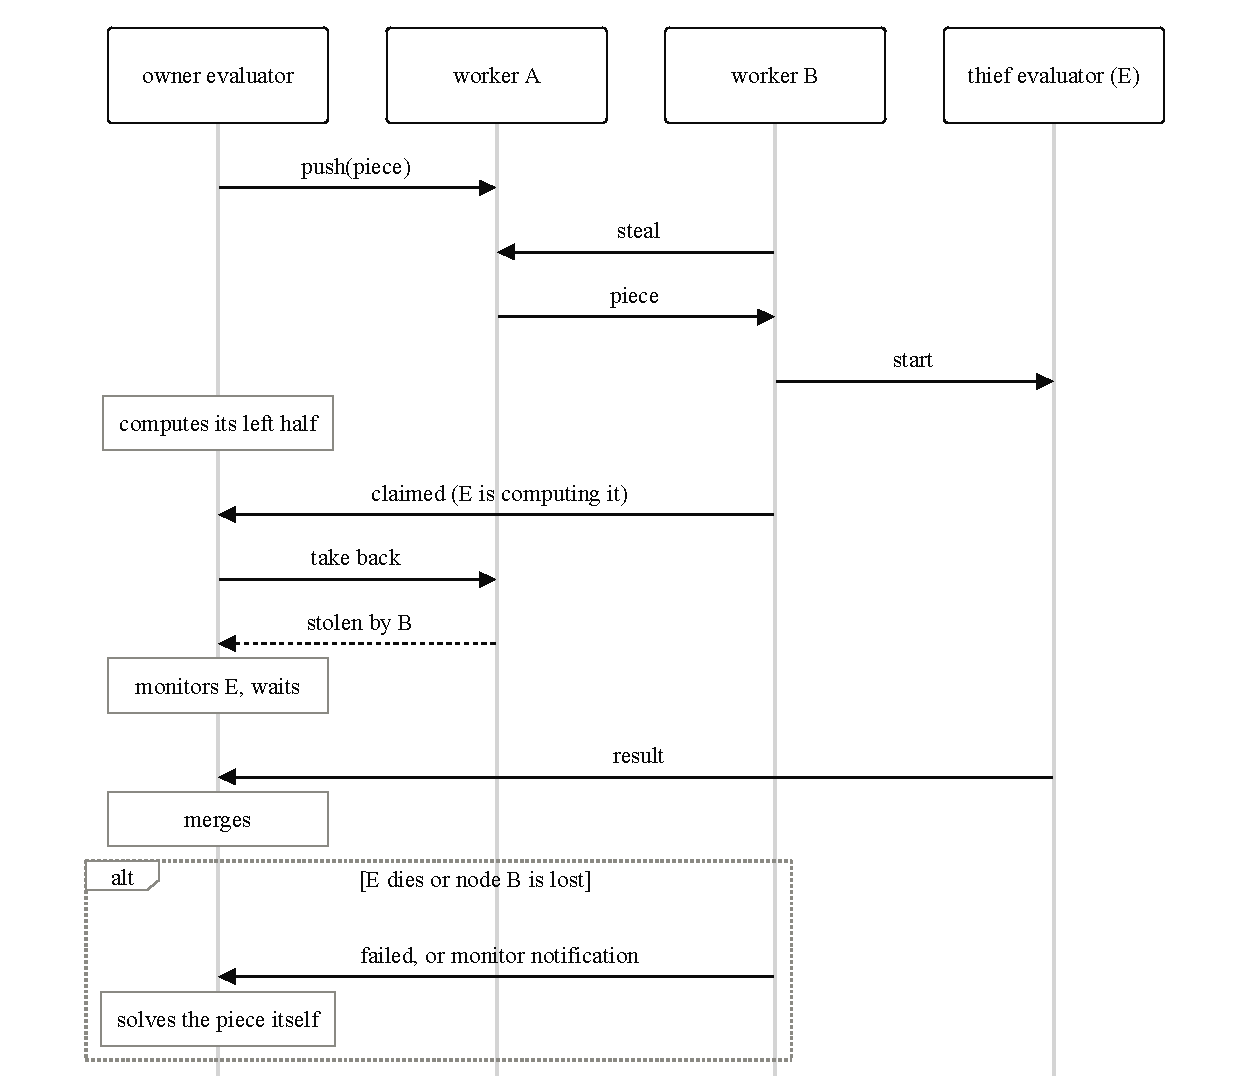
\includegraphics[width=0.68\textwidth]{figures/mermaid-steal.pdf}\else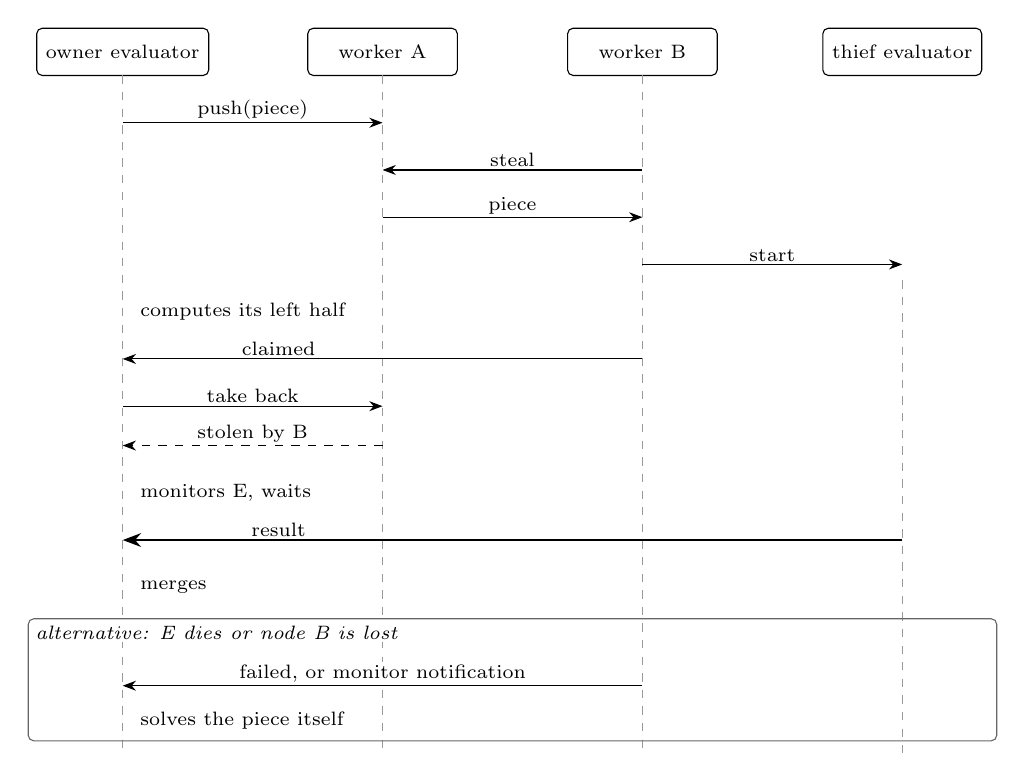
\begin{tikzpicture}[
      >=Stealth,
      hd/.style={draw, rounded corners=2pt, font=\scriptsize, minimum width=19mm, minimum height=6mm, fill=white},
      msg/.style={->, font=\scriptsize},
      lbl/.style={font=\scriptsize, fill=white, inner sep=1pt}]
    \def\yend{-8.9}
    \foreach \n/\x/\t in {o/0/owner evaluator, a/3.3/worker A, b/6.6/worker B, t/9.9/thief evaluator} {
      \node[hd] (h\n) at (\x, 0) {\t};
    }
    \draw[dashed, black!40] (0,-0.3) -- (0,\yend);
    \draw[dashed, black!40] (3.3,-0.3) -- (3.3,\yend);
    \draw[dashed, black!40] (6.6,-0.3) -- (6.6,\yend);
    \draw[dashed, black!40] (9.9,-2.9) -- (9.9,\yend);
    \draw[msg] (0,-0.9) -- node[lbl, above] {push(piece)} (3.3,-0.9);
    \draw[msg] (6.6,-1.5) -- node[lbl, above] {steal} (3.3,-1.5);
    \draw[msg] (3.3,-2.1) -- node[lbl, above] {piece} (6.6,-2.1);
    \draw[msg] (6.6,-2.7) -- node[lbl, above] {start} (9.9,-2.7);
    \node[font=\scriptsize, fill=white, right] at (0.1,-3.3) {computes its left half};
    \draw[msg] (6.6,-3.9) -- node[lbl, above, pos=0.7] {claimed} (0,-3.9);
    \draw[msg] (0,-4.5) -- node[lbl, above] {take back} (3.3,-4.5);
    \draw[msg, dashed] (3.3,-5.0) -- node[lbl, above] {stolen by B} (0,-5.0);
    \node[font=\scriptsize, fill=white, right] at (0.1,-5.6) {monitors E, waits};
    \draw[msg, thick] (9.9,-6.2) -- node[lbl, above, pos=0.8] {result} (0,-6.2);
    \node[font=\scriptsize, fill=white, right] at (0.1,-6.8) {merges};
    \draw[black!60, rounded corners=2pt] (-1.2,-7.2) rectangle (11.1,-8.75);
    \node[font=\scriptsize\itshape, anchor=north west, inner sep=1pt, fill=white] at (-1.15,-7.25) {alternative: E dies or node B is lost};
    \draw[msg] (6.6,-8.05) -- node[lbl, above, pos=0.5] {failed, or monitor notification} (0,-8.05);
    \node[font=\scriptsize, fill=white, right] at (0.1,-8.5) {solves the piece itself};
  \end{tikzpicture}
\fi
  \caption{Sequence diagram of a stolen piece. If the owner asks for its piece back before anyone steals it, it simply computes it. In the failure case, an error of the program is reported instead of recomputing, since it would occur again.}
  \label{fig:steal}
\end{figure}

\subsection{Behaviour}\label{behaviour}

\paragraph{Evaluators.}
An evaluator is stateless apart from the pieces it is waiting for.
%
When the interpreter meets a \texttt{dc}, the evaluator follows the logic of Listing~\ref{lst:solve}.
%
The same logic runs in the evaluator of a stolen piece, which is how a thief splits a large piece further and exposes its own halves to other nodes.
%
If an error interrupts the computation, each level first withdraws its own piece from the deque, so that a failed job leaves no work behind.

\begin{lstlisting}[float=tbp, caption={Simplified logic of an evaluator for a divide-and-conquer step.}, label={lst:solve}, captionpos=b]
solve(work):
  if small?(work.value): return base(work.value)
  [left, right] = split(work.value)
  push the right half as a new piece
  l = solve(left)
  case take_back(right piece):
    still in the deque -> r = solve(right)
    stolen by a thief  -> wait for the result:
                            result v           -> r = v
                            error of program   -> raise it again
                            evaluator/node lost -> r = solve(right)
  return merge(l, r)
\end{lstlisting}

\paragraph{Termination.}
A job ends when the evaluation of \texttt{main} returns.
%
Since every piece has an owner that waits for it before returning, the return of the first computation implies that every piece has been accounted for.
%
No termination detection protocol is therefore needed: the Dijkstra--Scholten algorithm~\cite{dijkstra1980termination}, listed among the optional extensions of the proposal, becomes unnecessary in this model.
%
The distinction between ``result available'', ``no local work'' and ``global termination'' collapses: the first is what the submitter observes, the second is a local condition used by workers to decide when to steal, and the third never has to be detected.

\paragraph{Workers.}
The worker is the only stateful component, and it changes state only in response to messages, one at a time (\cref{fig:worker}).
%
\begin{itemize}
  \item It starts evaluators for its own newest pieces while it has fewer running than a limit, by default the number of processor cores. Pieces beyond the limit stay in the deque, visible to thieves.
  \item It steals only when its deque is empty and it has spare capacity, with one request in flight at a time.
  \item After an unsuccessful request it waits before asking again, doubling the wait from 10~ms up to 100~ms with random jitter, and resetting it as soon as it obtains work.
  \item A stolen piece always gets an evaluator, even beyond the limit, since the node asked for it.
\end{itemize}

The limit is essential to the design: a node that started an evaluator for every piece as soon as it was pushed would never leave anything in its deque, and no work could ever be stolen.

\paragraph{Membership.}
The membership process of a node tries its seeds, once a second, until it knows at least one member.
%
From then on it spreads the member list by gossip: when it connects to a node, and every two or three seconds with random jitter, it asks a random connected node for its list and connects to the nodes it did not know.
%
This is an anti-entropy exchange: every node eventually knows every other, without a register and without relying on the automatic full mesh of the Erlang runtime, which the two-machine deployment disables.
%
A node that disappears is dropped from the list; a restarted node joins again through its seeds.
%
Since thieves choose victims among the connected nodes, a node that joins while a job runs starts stealing from it at once.

\begin{figure}
  \centering
  \ifmermaid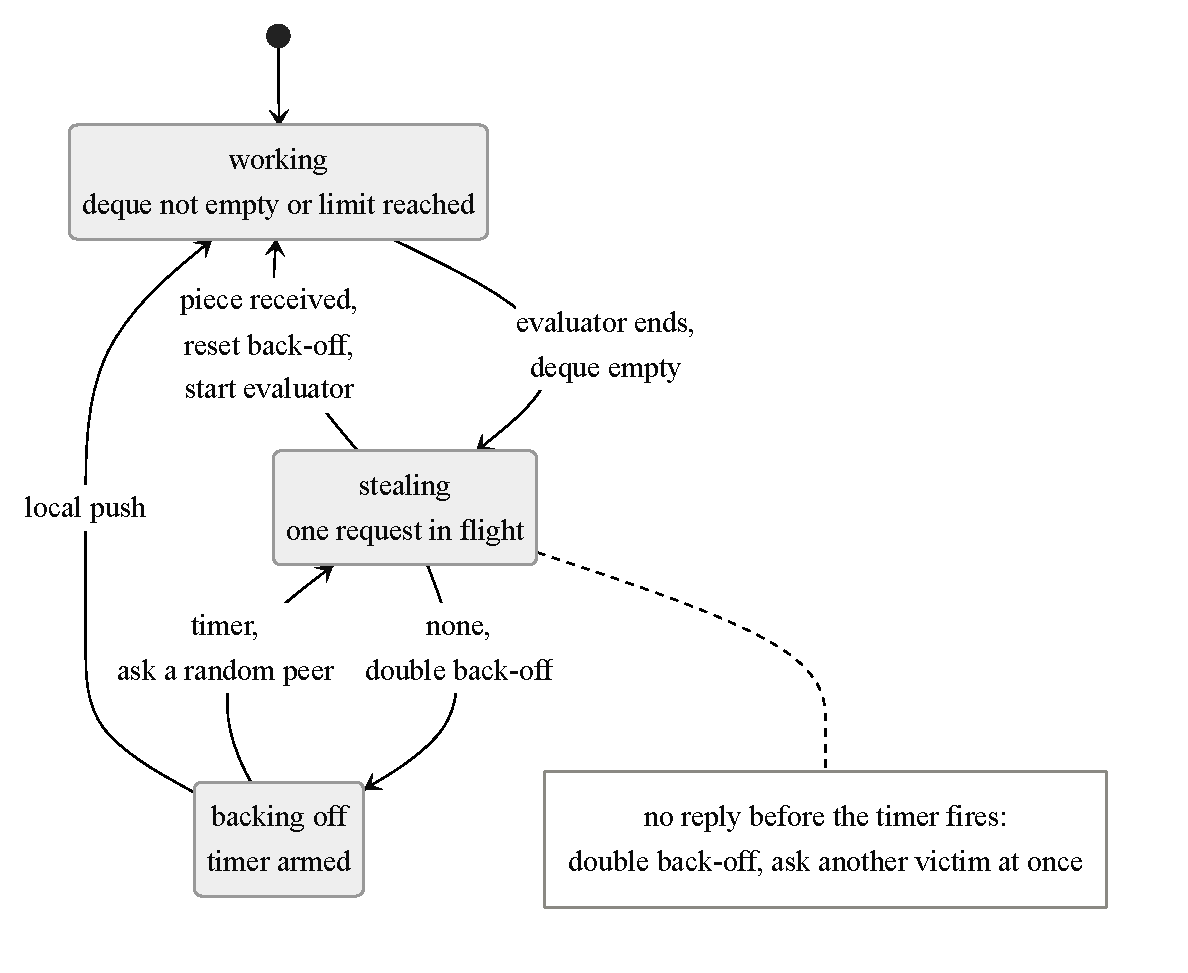
\includegraphics[width=0.6\textwidth]{figures/mermaid-worker.pdf}\else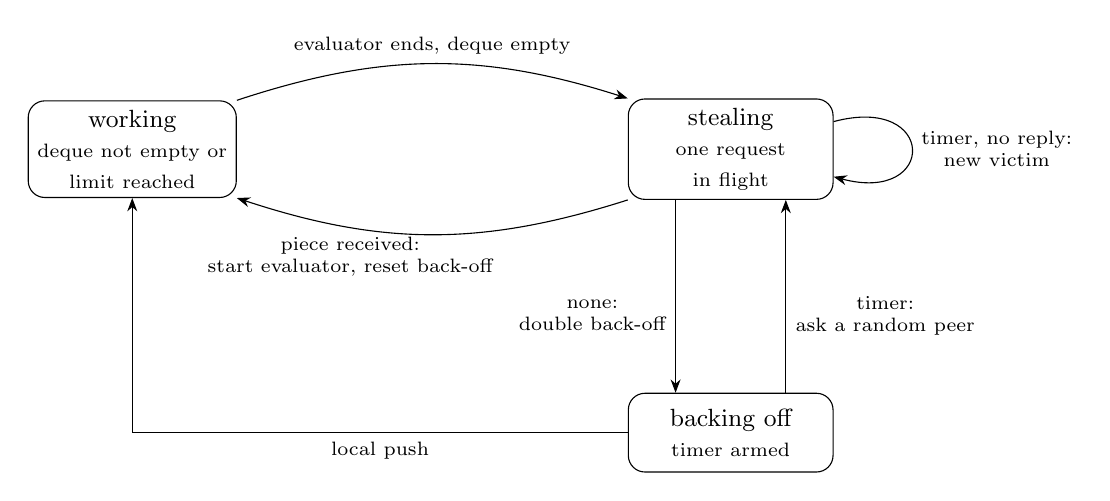
\begin{tikzpicture}[
    >=Stealth,
    st/.style={draw, rounded corners=6pt, minimum width=26mm, minimum height=10mm, align=center, font=\small},
    tr/.style={->, font=\scriptsize, align=center}]
  \node[st] (busy) at (0,0) {working\\\scriptsize deque not empty or\\\scriptsize limit reached};
  \node[st] (steal) at (7.6,0) {stealing\\\scriptsize one request\\\scriptsize in flight};
  \node[st] (wait) at (7.6,-3.6) {backing off\\\scriptsize timer armed};
  \draw[tr] (busy.north east) to[bend left=18] node[above] {evaluator ends, deque empty} (steal.north west);
  \draw[tr] (steal.south west) to[bend left=18] node[below, pos=0.72] {piece received:\\start evaluator, reset back-off} (busy.south east);
  \draw[tr] (steal) edge[loop right, looseness=5] node[right] {timer, no reply:\\new victim} (steal);
  \draw[tr] ([xshift=-7mm]steal.south) -- node[left, pos=0.6] {none:\\double back-off} ([xshift=-7mm]wait.north);
  \draw[tr] ([xshift=7mm]wait.north) -- node[right, pos=0.4] {timer:\\ask a random peer} ([xshift=7mm]steal.south);
  \draw[tr] (wait.west) -| node[below, pos=0.25] {local push} (busy.south);
\end{tikzpicture}
\fi
  \caption{Finite state machine of the worker's steal loop. In every state the worker also answers its own evaluators, steal requests from other nodes and requests for programs; a steal request that never gets an answer, because the victim failed, is treated as \emph{none} when the timer fires.}
  \label{fig:worker}
\end{figure}

\subsection{Data and Consistency Issues}\label{data-and-consistency-issues}

The system keeps no persistent data (\cref{concept}).
%
The only data shared between nodes is the program of a job.
%
It is immutable once the job is submitted, and each node caches it the first time it needs it, by asking the origin.
%
Every copy is therefore identical by construction, and no consistency protocol is needed.

Pieces are never shared: at any time a piece is in its creator's deque, held by exactly one evaluator, or finished.
%
All transitions happen inside the worker, which handles one message at a time, so a piece cannot be taken back by its owner and given to a thief at the same time.

Consistency of the \emph{results} comes from purity rather than from coordination.
%
Whichever node computes a piece, and however many times, it produces the same value, and the order of combination is fixed by the split.
%
The result of a job is therefore always equal to its sequential evaluation.

Since functions travel as closures, a piece carries every variable its functions captured: a function created where the input of the job is visible carries the whole input with every piece, even if it never uses it (\cref{implementation}).

\subsection{Fault-Tolerance}\label{fault-tolerance}

Fault tolerance is achieved through recomputation rather than replication.
%
\begin{itemize}
  \item \textbf{Unit of recovery:} the piece. The owner of a stolen piece still holds its data, and purity makes computing it again safe.
  \item \textbf{Failure detection:} process monitors, which the Erlang runtime delivers across machines. A monitor reports the death of a remote process, with its reason, or the loss of the connection to its node, detected by the runtime's distribution layer; no application-level heartbeat or timeout is used.
  \item \textbf{Reporting the cause:} the thief's worker, which monitors its evaluators anyway, sends the owner the reason why an evaluator died. This is needed because owners usually look at a stolen piece only after finishing their own half, when a monitor on an already dead process can only report that it no longer exists.
  \item \textbf{Program errors are not retried:} if a piece failed because of an error in the program, the owner raises the same error, since a deterministic program would fail again.
  \item \textbf{Crashes are retried once, locally:} for any other cause, a crashed process or a lost node, the owner computes the piece in its own process. A second failure then propagates normally, so recovery cannot loop.
  \item \textbf{Isolation:} evaluators are not linked to their worker, so a failing program never brings a node down.
\end{itemize}

The failure of the submitting node, and Byzantine failures, are outside the scope of the project.

\subsection{Availability}\label{availability}

Each node caches the program of a job the first time it meets a piece of that job, so the origin is asked at most once per node and per job.
%
Work stealing is the load balancing mechanism: busy nodes are never interrupted, idle nodes pull work from randomly chosen peers.
%
In the presence of a \textbf{network partition}:
%
\begin{itemize}
  \item workers only choose victims among the nodes they can reach, so each side continues with the work it can see;
  \item pieces held by thieves on the other side are treated by their owners as lost, and recomputed;
  \item the side that holds the submitting node completes the job, possibly more slowly, and results computed on the other side are discarded.
\end{itemize}

In terms of the CAP theorem, a job gives up speed rather than correctness: it never returns a partial or wrong result, and it keeps making progress as long as the submitting node is alive.

\subsection{Security}\label{security}

Security is intentionally outside the scope of this project, and the system assumes a trusted private network: the only authentication is the shared secret (\emph{cookie}) required by the Erlang runtime to connect two nodes, there is no authorization and there are no roles, and traffic is not encrypted.

Pieces of work are data interpreted by a language that cannot perform any action other than computing a value, so a piece cannot by itself execute arbitrary code on a thief.
%
The Erlang distribution layer, however, grants a connected node full control over the others, so the cookie must be treated as a password and the cluster must not be exposed to untrusted networks.

\section{Implementation}\label{implementation}

\begin{itemize}
  \item \textbf{Network Protocol:} all communication uses the distribution protocol of the Erlang runtime over TCP~\cite{erlangdistributed}. It provides reliable, ordered delivery between each pair of processes, and failure notifications between processes on different machines, which is what the steal protocol and the recovery mechanism rely on.

  \item \textbf{Data Representation:} messages are Erlang terms, encoded by the runtime in its external term format. Parsed programs are nested lists of symbols, and closures are tuples of parameter names, body and captured variables. Since no compiled code ever crosses a node boundary, the project needs no serialization code.

  \item \textbf{Persistence and authorization:} none; all state is in memory, and the only authentication is the runtime cookie (\cref{security}).
\end{itemize}

\paragraph{Mapping of the design.}
\begin{itemize}
  \item \textbf{Worker:} an OTP \texttt{GenServer} registered under a fixed name, so that the worker of any node is reachable by its name and the name of the node. All exchanges between workers are asynchronous: a worker never waits for another node, and is therefore always free to answer its own evaluators. The only synchronous remote request, fetching a program, is made by evaluators.
  \item \textbf{Evaluators:} processes started under an OTP \texttt{Task.Supervisor}.
  \item \textbf{Membership:} a separate \texttt{GenServer} that exchanges member lists with plain messages; connection attempts run in separate processes, since connecting to an unreachable node can take seconds.
  \item \textbf{Dashboard:} a collector that asks every node for its counters twice a second, with a short timeout so that a lost node cannot block it, and a small HTTP server written directly on TCP sockets, which serves a page and the collected data as JSON. A node that stops answering is kept on the page and marked as down, so failures stay visible.
  \item \textbf{Schedulers:} the interpreter delegates each \texttt{dc} to a scheduler. Three schedulers share the same definition of \texttt{dc}: a \emph{sequential} one, used as the reference for correctness; a \emph{local} one, which runs halves on separate processes of the same node; and the \emph{distributed} one described in \cref{design}.
  \item \textbf{Interpreter:} a tree-walking interpreter. Calls in tail position are executed without growing the stack, so loops written as recursive functions run in constant memory.
\end{itemize}

\paragraph{Size of pieces.}
Since closures carry the variables they captured (\cref{data-and-consistency-issues}), the functions that the library passes to \texttt{dc} are created in definitions where only what they need is visible.
%
The difference was measured on a parallel map over 100\,000 integers: when the base case of \texttt{pmap} was created inside its body, where the input list was visible, every piece carried the whole input, about 500~kB; created in a separate definition it carries 341 bytes, and the job on one node became a third faster.
%
Functions written by the user inside \texttt{main} still capture its argument, which is the input of the job, so programs should define the functions they pass to parallel operations at top level (\cref{user-guide}).

\subsection{Technological Details}\label{technological-details}

The system runs on Elixir 1.20 and Erlang/OTP 29.
%
Besides the OTP behaviours and the Erlang distribution described above, it uses the OTP \texttt{peer} module to start real additional nodes during automated tests, ExUnit as testing framework, and Docker Compose for the containerized deployment.
%
Nodes are configured on the command line and through environment variables (\cref{tab:config}).

\begin{table}
  \centering
  \small
  \begin{tabularx}{\textwidth}{@{}lYl@{}}
    \toprule
    Parameter & Description & Default \\
    \midrule
    node name & unique name of the node (\texttt{--sname} or \texttt{--name}) & required \\
    cookie & shared secret of the cluster (\texttt{--cookie}) & required \\
    \texttt{THUNK\_PEERS} & comma-separated seeds: existing nodes to join through; one reachable seed is enough & none \\
    \texttt{THUNK\_LIMIT} & evaluators the node runs from its own deque & processor cores \\
    \bottomrule
  \end{tabularx}
  \caption{Configuration of a node.}
  \label{tab:config}
\end{table}

\paragraph{Module structure:}
\begin{lstlisting}
src/thunk_lexer.xrl, thunk_parser.yrl   # tokens and grammar
lib/thunk/eval.ex                       # interpreter
lib/thunk/primitives.ex                 # the thirteen primitive operations
lib/thunk/scheduler/{sequential,local,distributed}.ex
lib/thunk/worker.ex                     # deque, steal loop, program cache
lib/thunk/cluster.ex                    # submitting jobs to the cluster
lib/thunk/membership.ex                 # seeds and gossip of the member list
lib/thunk/dashboard.ex                  # collector and HTTP server
lib/mix/tasks/thunk.demo.ex             # command-line demonstrations
priv/prelude.thunk                      # standard library, in Thunk
priv/demos/*.thunk                      # demonstration programs, in Thunk
\end{lstlisting}

\section{Validation}\label{validation}

\subsection{Automatic Testing}\label{automatic-testing}

\paragraph{Test infrastructure.}
Tests are written with ExUnit and cover the parser, the interpreter, the library, the schedulers, the worker and the cluster.
%
Three techniques are used throughout:
%
\begin{itemize}
  \item \textbf{Oracle testing:} the sequential scheduler is the reference. Every program must give identical results under the other schedulers, and the demonstration programs are compared with native Elixir implementations on random inputs.
  \item \textbf{Real multi-node tests:} the test process turns itself into a distributed node and starts additional Erlang nodes with the OTP \texttt{peer} module, each running the Thunk application and connecting back. These tests exercise the actual protocol between nodes, not a simulation.
  \item \textbf{Fault injection:} tests start fake thieves that take a piece and die, or report a program error, and multi-node tests stop a real node in the middle of a job.
\end{itemize}

\paragraph{Test coverage.}
\Cref{tab:tests} maps the requirements of \cref{requirements} to the tests that check them.

\begin{table}
  \centering
  \small
  \begin{tabularx}{\textwidth}{@{}l>{\hsize=1.7\hsize}Y>{\hsize=0.75\hsize}Y>{\hsize=0.55\hsize}Y@{}}
    \toprule
    Requirement & What is checked & Test module & Kind \\
    \midrule
    FR1 & every special form, scoping, order of evaluation and the error for each misuse; a loop of a million iterations in constant memory; list, sorting and parallel library against native results & \texttt{parser}, \texttt{eval}, \texttt{primitives}, \texttt{prelude} & unit, oracle \\
    FR2 & base case, split and merge order, nested \texttt{dc}, errors for a threshold that is not a boolean or a split without two parts & \texttt{scheduler/} \texttt{sequential} & unit \\
    FR3 & oldest piece to thieves, take-back, counters; a mergesort submitted on a node that computes nothing returns the sequential result and the other nodes report steals & \texttt{worker}, \texttt{cluster} & unit, multi-node \\
    FR4 & a job using a definition that exists only on the submitter completes on the cluster; programs are fetched by job and cached & \texttt{cluster}, \texttt{worker} & multi-node \\
    FR5 & an error in a piece computed on another node is raised at the submitter; a program error reported by a thief is not retried & \texttt{cluster}, \texttt{scheduler/} \texttt{distributed} & multi-node, fault injection \\
    FR6 & a fake thief takes a piece and dies and the owner solves it; a real node with high capacity is stopped in the middle of a job, the result is exact and the survivors report recovered pieces & \texttt{scheduler/} \texttt{distributed}, \texttt{cluster} & fault injection, multi-node \\
    FR7 & mergesort, word count and both images give identical results under the sequential, local and distributed schedulers, and equal native implementations & \texttt{demo}, \texttt{cube}, \texttt{mandelbrot} & oracle \\
    FR8 & with full mesh disabled, B seeded with A and C with B all end up connected; a node joining during a job takes part in it & \texttt{membership} & multi-node \\
    Determinism & the same result for every scheduler and any local capacity & \texttt{scheduler/local}, \texttt{demo} & oracle \\
    Observability & rates from counters, a node that disappears shown as down, page and data served over HTTP & \texttt{dashboard} & unit, multi-node \\
    Piece size & the functions carried by the pieces of \texttt{pmap} do not capture the input list & \texttt{prelude} & unit \\
    \bottomrule
  \end{tabularx}
  \caption{Requirements and the tests that check them. Module names are relative to \texttt{test/thunk/}; multi-node tests start real additional nodes, fault injection tests kill a thief or a node during a job.}
  \label{tab:tests}
\end{table}

\paragraph{How to run.}
The whole suite, including the multi-node tests, runs with \texttt{mix test}; formatting and warnings are checked with \texttt{mix format --check-formatted} and \texttt{mix compile --warnings-as-errors}.
%
The multi-node tests require the Erlang name service (\texttt{epmd}), which the test helper starts if needed; if distribution cannot be started, they are skipped with a message.

\subsection{Experimental Evaluation}\label{sec:experiments}

\paragraph{Setup.}
The first environment is a laptop with 12 hardware threads running Windows 11 and Docker Desktop, with three Thunk nodes in containers and a fourth node, inside the first container, that submits jobs without computing any piece itself, so that all work below the first split has to be stolen.
%
The second is the laptop together with a virtual private server with 4 cores running Debian, about 22~ms away and also hosting other services; to make the two machines comparable, the laptop node was limited to 4 schedulers, and a third node on the laptop submitted the jobs.
%
The server was reached through an SSH tunnel bound to its loopback interface, so no port was exposed to the Internet, and automatic full-mesh connection was disabled so that the server never tries to connect to the private addresses of the laptop.
%
Four workloads were used: mergesort of random integers, word count of random text, a raytraced cube and the Mandelbrot set, both images computed row by row in fixed-point arithmetic.
%
Times and counters come from the output of the demonstration command.
%
Since the containers of the first environment share the processors of one machine, that environment measures the \emph{overhead} of distribution rather than speed-up; the second measures the effect of adding a machine.

\paragraph{Correctness.}
Every run of every experiment reported a correct result: sorted lists equal to the native sort, word counts equal to the native count, and images identical byte for byte whatever the scheduler, the number of nodes and the size of the pieces (\cref{fig:images}).

\begin{figure}
  \centering
  
\includegraphics[width=0.36\textwidth]{figures/cube.png}\hspace{4mm}
  
\includegraphics[width=0.42\textwidth]{figures/mandelbrot.png}
  \caption{The two image workloads, the raytraced cube at $1280\times960$ and the Mandelbrot set at $640\times480$, both computed by the laptop and the server together.}
  \label{fig:images}
\end{figure}

\paragraph{Overhead and speed-up.}
\Cref{fig:time} compares the schedulers on one machine and the cluster on one and on two machines.
%
On the laptop, parallel execution is four to five times faster than sequential execution, and the cluster of three containers costs nothing measurable on the sort and between a fifth and a third more time on the small image: this is the price of stealing, copying pieces between containers and returning results.
%
On two machines, with five runs per configuration after a warm-up run, the second machine makes jobs faster, the image 1.5 times and the sort 1.2 times; the server alone is slower than the laptop alone, since it also serves other applications and every piece it computes crosses the network.
%
The division of work between the machines was not configured anywhere and adapts to the cost of communication: the server took more than half of the pieces of the image, which are cheap to send and expensive to compute, but only a quarter of the pieces of the sort, which carry the list they sort across the 22~ms link.

\begin{figure}
  \centering
  % Job time under each scheduler, on the same machine. One series per panel.
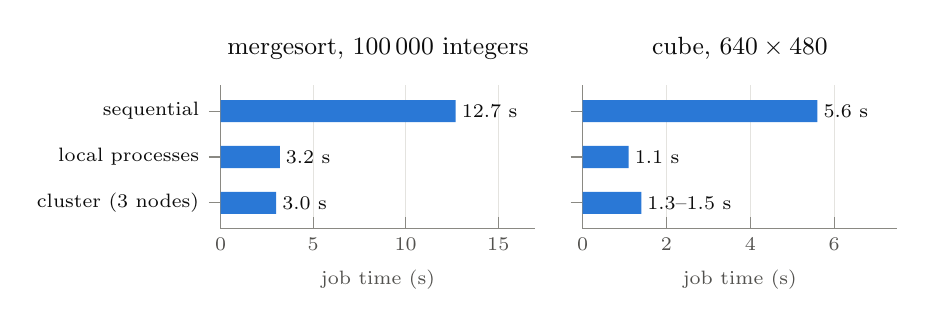
\begin{tikzpicture}
  \begin{groupplot}[
      thunkplot, thunkhbar,
      group style={group size=2 by 1, horizontal sep=6mm, yticklabels at=edge left},
      width=0.46\textwidth, height=34mm,
      symbolic y coords={clu, loc, seq},
      ytick={clu, loc, seq},
      yticklabels={cluster (3 nodes), local processes, sequential},
      enlarge y limits=0.28,
      xlabel={job time (s)},
    ]
    \nextgroupplot[title={mergesort, 100\,000 integers}, xmin=0, xmax=17]
    \addplot[fill=series1] coordinates {
      (12.7,seq) [12.7 s]
      (3.2,loc) [3.2 s]
      (3.0,clu) [3.0 s]
    };
    \nextgroupplot[title={cube, $640\times480$}, xmin=0, xmax=7.5]
    \addplot[fill=series1] coordinates {
      (5.6,seq) [5.6 s]
      (1.1,loc) [1.1 s]
      (1.4,clu) [1.3--1.5 s]
    };
  \end{groupplot}
\end{tikzpicture}


  \vspace{1mm}
  % Median job time over five runs on a laptop node and a VPS node, each with
% four schedulers, 22 ms apart. The configuration using both machines is
% highlighted; the single-machine configurations are the reference.
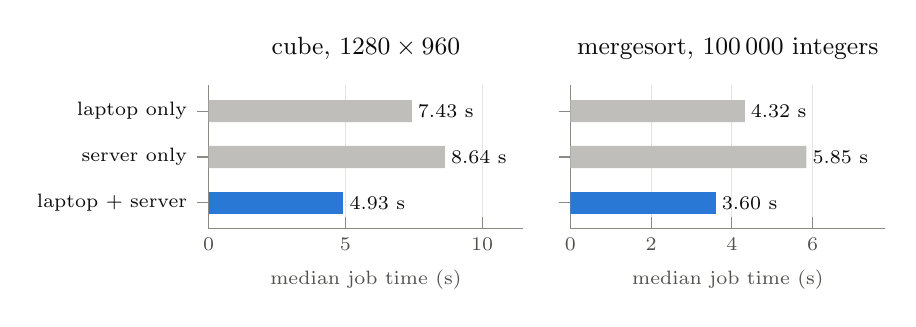
\begin{tikzpicture}
  \begin{groupplot}[
      thunkplot, thunkhbar,
      group style={group size=2 by 1, horizontal sep=6mm, yticklabels at=edge left},
      width=0.46\textwidth, height=34mm,
      symbolic y coords={both, vps, lap},
      ytick={both, vps, lap},
      yticklabels={laptop + server, server only, laptop only},
      enlarge y limits=0.28,
      every axis plot/.append style={/pgf/bar shift=0pt},
      xlabel={median job time (s)},
    ]
    \nextgroupplot[title={cube, $1280\times960$}, xmin=0, xmax=11.5]
    \addplot[fill=axisline!55] coordinates {(7.43,lap) [7.43 s] (8.64,vps) [8.64 s]};
    \addplot[fill=series1] coordinates {(4.93,both) [4.93 s]};
    \nextgroupplot[title={mergesort, 100\,000 integers}, xmin=0, xmax=7.8]
    \addplot[fill=axisline!55] coordinates {(4.32,lap) [4.32 s] (5.85,vps) [5.85 s]};
    \addplot[fill=series1] coordinates {(3.60,both) [3.60 s]};
  \end{groupplot}
\end{tikzpicture}

  \caption{Job time. Top: the three schedulers on the same machine, so that the difference between the cluster and local processes is the cost of distribution. Bottom: median of five runs with one machine and with two machines 22~ms apart, each running a node with four schedulers.}
  \label{fig:time}
\end{figure}

\paragraph{Irregular work.}
In the workloads above, pieces of the same size cost about the same.
%
Work stealing is designed above all for the opposite case, in which nobody can tell in advance which pieces are expensive: in the Mandelbrot image the rows that cross the set cost up to 17 times more than the rows far from it, while the rows of the cube differ by a factor of two.
%
\Cref{fig:mandelbrot-pieces} shows the image computed on the two machines with pieces of different sizes.
%
With a few large pieces the two machines are more than twice as slow as the laptop alone: each piece is solved by a single process, most processors stay idle, and the job waits for whoever received an expensive middle piece, in the worst case the slower machine.
%
As the pieces become smaller, idle processors keep stealing, the expensive rows are spread over both machines, and with pieces of three rows the two machines beat the laptop alone.
%
The cube, whose time hardly changed with the size of the pieces, shows the contrast: when the cost of the work is uneven, dividing it finely and letting idle machines take it is what balances it, without anyone knowing where the expensive parts are.

\begin{figure}
  \centering
  % Mandelbrot 640x480 on laptop + server with different piece sizes, median
% of three runs; the laptop alone (fine pieces) is the reference.
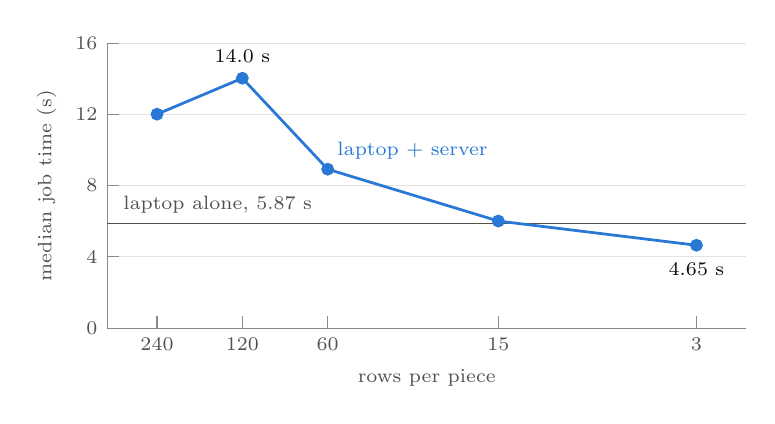
\begin{tikzpicture}
  \begin{axis}[
      thunkplot,
      width=0.8\textwidth, height=52mm,
      xmode=log, x dir=reverse,
      xmin=2, xmax=360,
      xtick={3,15,60,120,240},
      xticklabels={3,15,60,120,240},
      xlabel={rows per piece},
      ymin=0, ymax=16,
      ytick={0,4,8,12,16},
      ymajorgrids,
      ylabel={median job time (s)},
    ]
    \draw[refline] (axis cs:360,5.87) -- (axis cs:2,5.87)
      node[pos=0.01, anchor=south west, font=\scriptsize, text=textsecondary] {laptop alone, 5.87 s};
    \addplot[thunkline, color=series1] coordinates {(240,12.01) (120,14.03) (60,8.92) (15,6.01) (3,4.65)};
    \node[font=\scriptsize, anchor=south, yshift=2pt, text=textprimary] at (axis cs:120,14.03) {14.0 s};
    \node[font=\scriptsize, anchor=north, yshift=-3pt, text=textprimary] at (axis cs:3,4.65) {4.65 s};
    \node[font=\scriptsize, anchor=south west, text=series1] at (axis cs:60,8.92) {laptop + server};
  \end{axis}
\end{tikzpicture}

  \caption{The Mandelbrot image computed by the laptop and the server together, with pieces from 240 down to 3 rows; median of three runs. The reference line is the laptop alone with small pieces.}
  \label{fig:mandelbrot-pieces}
\end{figure}

\paragraph{Granularity.}
The threshold decides how many pieces a job is divided into, and therefore how much work there is to share and how many steals are needed.
%
\Cref{fig:granularity} shows mergesort of 100\,000 integers on the cluster at four thresholds.
%
With coarse pieces there are too few of them to keep all nodes busy and the job is almost as slow as a sequential one; with very fine pieces the cost of creating, exposing, stealing and combining thousands of pieces exceeds the useful work and the job becomes slower than a sequential one; the best results lie in between.
%
The number of steals, instead, stays between 14 and 33 while the pieces grow from 31 to almost two thousand, as predicted for randomized work stealing~\cite{blumofe1999scheduling}: thieves take the largest piece available, so a few steals give each node a large share of the work, which it then splits and computes locally.
%
The word count workload adds a caveat: the parallel part of a job must last long enough for thieves to arrive, and on a small text the sequential splitting into words dominated and nothing was stolen.

\begin{figure}
  \centering
  % Mergesort of 100000 integers on the cluster at four thresholds. Two panels
% on a shared threshold axis instead of one plot with two y scales.
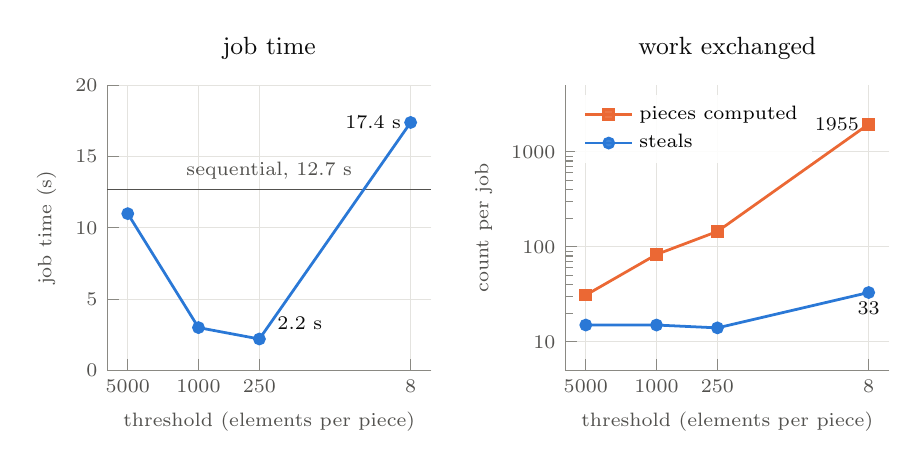
\begin{tikzpicture}
  \begin{groupplot}[
      thunkplot,
      group style={group size=2 by 1, horizontal sep=17mm},
      width=0.47\textwidth, height=52mm,
      xmode=log, x dir=reverse,
      xmin=5, xmax=8000,
      xtick={8,250,1000,5000},
      xticklabels={8,250,1000,5000},
      xlabel={threshold (elements per piece)},
      grid=major,
    ]
    \nextgroupplot[
      title={job time},
      ymin=0, ymax=20,
      ylabel={job time (s)},
    ]
    \draw[refline] (axis cs:8000,12.7) -- (axis cs:5,12.7)
      node[pos=0.5, above, font=\scriptsize, text=textsecondary] {sequential, 12.7 s};
    \addplot[thunkline, color=series1] coordinates {(5000,11.0) (1000,3.0) (250,2.2) (8,17.4)};
    \node[font=\scriptsize, anchor=south west, xshift=3pt, text=textprimary] at (axis cs:250,2.2) {2.2 s};
    \node[font=\scriptsize, anchor=east, text=textprimary] at (axis cs:8,17.4) {17.4 s};

    \nextgroupplot[
      title={work exchanged},
      ymode=log, ymin=5, ymax=5000,
      ytick={10,100,1000},
      yticklabels={10,100,1000},
      ylabel={count per job},
      legend style={at={(0.03,0.97)}, anchor=north west},
    ]
    \addplot[thunkline, color=series2, mark=square*] coordinates {(5000,31) (1000,83) (250,145) (8,1955)};
    \addlegendentry{pieces computed}
    \addplot[thunkline, color=series1] coordinates {(5000,15) (1000,15) (250,14) (8,33)};
    \addlegendentry{steals}
    \node[font=\scriptsize, anchor=east, text=textprimary] at (axis cs:8,1955) {1955};
    \node[font=\scriptsize, anchor=north, text=textprimary] at (axis cs:8,33) {33};
  \end{groupplot}
\end{tikzpicture}

  \caption{Mergesort of 100\,000 integers on the cluster, from coarse pieces (left) to very fine pieces (right). Left: job time, with the sequential time as reference. Right: pieces computed by the nodes and steals needed, on a logarithmic scale.}
  \label{fig:granularity}
\end{figure}

\paragraph{Failure recovery.}
A crash was simulated by killing one of the three computing containers two seconds into the rendering of a $1280\times960$ image (\cref{fig:recovery}).
%
In both runs the job completed and the image was identical, byte for byte, to the one rendered without failures; the lost pieces were recomputed by their owners.
%
Recovery is \emph{lazy}: the loss of the node was logged about eight seconds before the owner of a lost piece noticed it, because an owner looks at a stolen piece only after finishing its own half, so the job waited for work that no longer existed.
%
The same experiment on the two machines, killing the server node three seconds into the job, completed in 6.6 and 10.5~s instead of about 4.9~s, again with identical images; there the loss was detected as soon as the connection closed, because the owner of the first lost piece was already waiting for it.

\begin{figure}
  \centering
  % Rendering of a 1280x960 image, with and without a node killed after two
% seconds. One series; the labels carry the number of recomputed pieces.
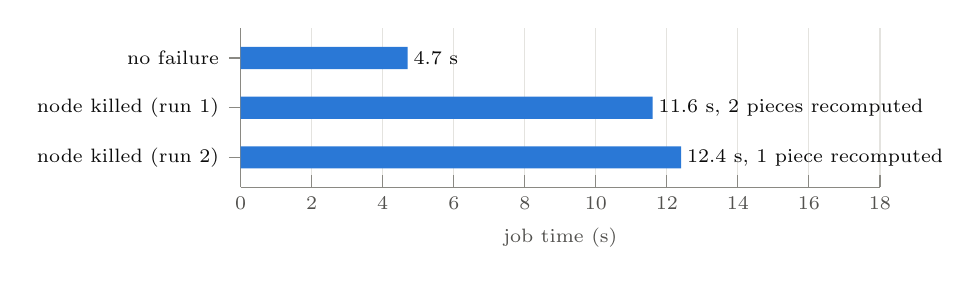
\begin{tikzpicture}
  \begin{axis}[
      thunkplot, thunkhbar,
      width=0.8\textwidth, height=36mm,
      symbolic y coords={k2, k1, ok},
      ytick={k2, k1, ok},
      yticklabels={node killed (run 2), node killed (run 1), no failure},
      enlarge y limits=0.3,
      xmin=0, xmax=18,
      xlabel={job time (s)},
    ]
    \addplot[fill=series1] coordinates {
      (4.7,ok) [4.7 s]
      (11.6,k1) [11.6 s, 2 pieces recomputed]
      (12.4,k2) [12.4 s, 1 piece recomputed]
    };
  \end{axis}
\end{tikzpicture}

  \caption{Rendering of a $1280\times960$ image on the cluster, without failures and with a node killed after two seconds. In both runs with a failure the image is identical to the reference.}
  \label{fig:recovery}
\end{figure}

\subsection{Acceptance Testing}\label{acceptance-test}\label{sec:acceptance}

Manual acceptance testing was performed on the Docker Compose cluster, for scenarios that depend on the deployed system as a whole:
%
\begin{itemize}
  \item \textbf{Demonstrations:} the four workloads were submitted from a node inside the cluster, checking that every run reports a correct result and that the counters of all nodes change; the rendered images and a ten-frame orbit animation around the cube were inspected.
  \item \textbf{Node crash:} a container was killed during a job with \texttt{docker compose kill}, and the result compared with a run without failures (\cref{fig:recovery}).
  \item \textbf{Dashboard:} the live page was watched while jobs ran and while a node was killed, checking that the rates move and that the node is marked as down.
\end{itemize}
%
These scenarios need Docker and visual inspection; their automated counterparts are the multi-node tests.

\section{Deployment}\label{deployment}

\subsection{Requirements and Setup}

The cluster needs Docker and Docker Compose; running a node or the tests outside containers needs Elixir 1.20 and Erlang/OTP 29, which on Windows without administrator rights can be installed with Scoop.
%
A single image is built from the repository: it compiles the project and starts a node whose name, cookie and peers are taken from environment variables.
\begin{lstlisting}
git clone <repository url> && cd thunk
mix compile && mix test          # outside containers
docker compose up -d --build     # the cluster
docker compose logs
\end{lstlisting}

\subsection{Docker Compose Design}

The Compose file declares three services, \texttt{node1}, \texttt{node2} and \texttt{node3}, built from the same image (\cref{fig:compose}).
%
Each service has a host name equal to its service name, lists the other two as peers and shares the same cookie.
%
Short node names are used, because the Erlang runtime rejects long names whose host has no dot, as is the case for container host names, and nodes retry their seeds every second until one answers, so they can start in any order.
%
A fourth service, \texttt{joiner}, is disabled by default (Compose profile \texttt{join}); it has no fixed host name and only \texttt{node1} as seed, so it can be scaled to add any number of nodes to the running cluster.
%
The submitting node and the dashboard are short-lived nodes started inside the first container, whose port 4000 is published to the host.

\begin{figure}
  \centering
  \resizebox{0.85\linewidth}{!}{%
  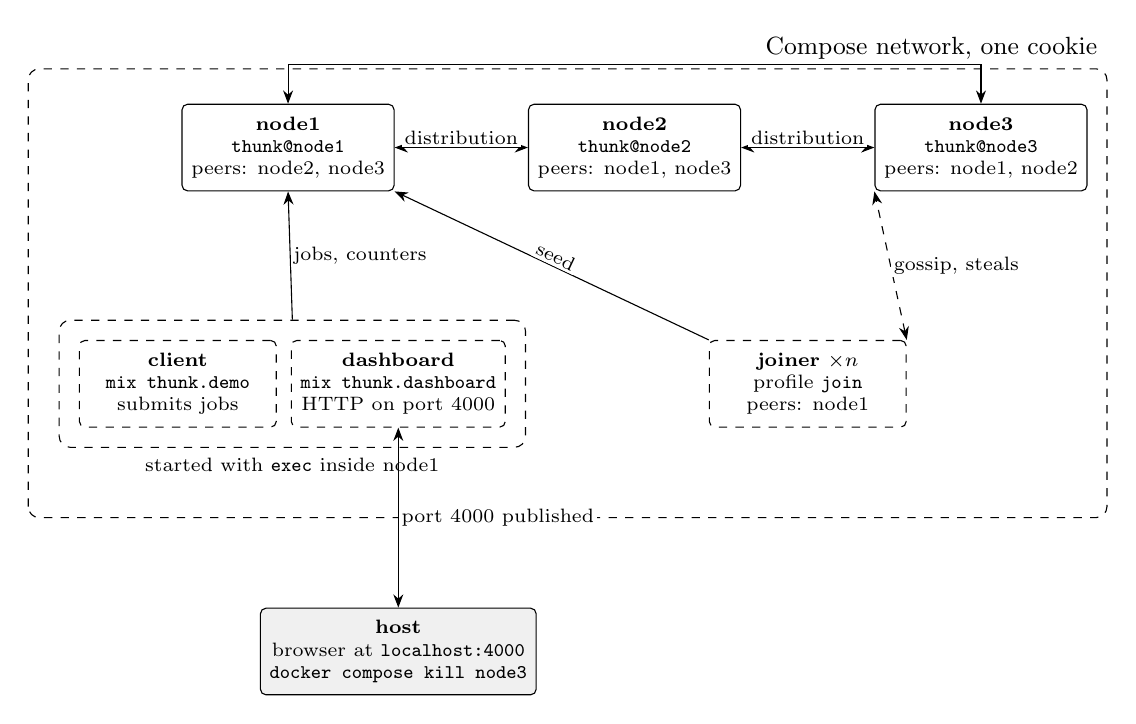
\begin{tikzpicture}[
      >=Stealth, font=\scriptsize,
      svc/.style={draw, rounded corners=2pt, minimum width=25mm, minimum height=11mm, align=center, fill=white},
      opt/.style={svc, dashed},
      grp/.style={draw, dashed, rounded corners=4pt},
      lbl/.style={font=\scriptsize, fill=white, inner sep=1pt}]
    \node[svc] (n1) at (0,0) {\textbf{node1}\\\texttt{thunk@node1}\\peers: node2, node3};
    \node[svc] (n2) at (4.4,0) {\textbf{node2}\\\texttt{thunk@node2}\\peers: node1, node3};
    \node[svc] (n3) at (8.8,0) {\textbf{node3}\\\texttt{thunk@node3}\\peers: node1, node2};
    \node[opt] (c) at (-1.4,-3) {\textbf{client}\\\texttt{mix thunk.demo}\\submits jobs};
    \node[opt] (d) at (1.4,-3) {\textbf{dashboard}\\\texttt{mix thunk.dashboard}\\HTTP on port 4000};
    \node[opt] (j) at (6.6,-3) {\textbf{joiner} $\times n$\\profile \texttt{join}\\peers: node1};
    \node[grp, inner sep=2.5mm, fit=(c)(d), label={[font=\scriptsize]below:started with \texttt{exec} inside node1}] (inside) {};
    \draw[<->] (n1) -- node[lbl, above] {distribution} (n2);
    \draw[<->] (n2) -- node[lbl, above] {distribution} (n3);
    \draw[<->] (n1.north) -- ++(0,0.5) -| (n3.north);
    \draw[->] (j.north west) -- node[lbl, above, sloped] {seed} (n1.south east);
    \draw[<->, dashed] (j.north east) -- node[lbl, right] {gossip, steals} (n3.south west);
    \draw[->] (inside.north) -- node[lbl, right] {jobs, counters} (n1.south);
    \draw[grp] (-3.3,-4.7) rectangle (10.4,1.0) node[pos=1, anchor=south east, font=\small] {Compose network, one cookie};
    \node[svc, fill=black!6] (host) at (1.4,-6.4) {\textbf{host}\\browser at \texttt{localhost:4000}\\\texttt{docker compose kill node3}};
    \draw[<->] (host) -- node[lbl, right] {port 4000 published} (d);
  \end{tikzpicture}}
  \caption{Docker Compose deployment. Three permanent services form the cluster; the optional \texttt{joiner} service can be scaled to add nodes; the submitter and the dashboard run as short-lived nodes inside the first container. Dashed boxes are optional or short-lived.}
  \label{fig:compose}
\end{figure}

After startup, each node logs the other nodes as they connect and as they become members; when a job is submitted, the counters of the nodes show pieces stolen and evaluated; when a node is stopped, the others log its disconnection.

\section{User Guide}\label{user-guide}

\subsection{Writing a Program}

A program is a sequence of definitions with a \texttt{main} of one argument, and may use every function of the prelude.
%
For example, the sum of squares of a list computed in parallel:
\begin{lstlisting}
def square(x) = x * x
def small?(v) = length(v) < 1000
def main(xs) = reduce(add, pmap(square, xs, small?), small?)
\end{lstlisting}
%
Functions passed to parallel operations should be defined at top level, as here, so that pieces of work carry only the data they need.

The program is submitted from an Elixir shell on any node:
\begin{lstlisting}
ctx = Thunk.Cluster.load(File.read!("sum.thunk"))
Thunk.Cluster.run(ctx, Enum.to_list(1..100_000))
\end{lstlisting}

\subsection{Running the Demonstrations}

\begin{lstlisting}
docker compose exec node1 sh -c 'elixir --sname client \
  --cookie thunk-demo -S mix thunk.demo cube --width 640 --height 480'
\end{lstlisting}

The demonstration command accepts \texttt{mergesort}, \texttt{wordcount}, \texttt{cube} or \texttt{mandelbrot}, and options for the size of the input, the threshold, the number of repetitions, the scheduler, and the number of pieces the submitting node may compute itself.
%
The cube accepts \texttt{--frames} to render an orbit as an animated image.
%
Each run prints its time, the outcome of the check, and the counters of every node:
\begin{lstlisting}
peers: [:thunk@node2, :thunk@node3]
run 1: cube 640x480 angle=3798 threshold=8 ok 1253 ms
  client@node1: steals=0 stolen_from=3 evaluated=0 recovered=0
  thunk@node2: steals=20 stolen_from=9 evaluated=151 recovered=0
  ...
\end{lstlisting}

\paragraph{Adding nodes to a running cluster.}
The following command starts two more nodes, which join through \texttt{node1}, learn the other members by gossip, and take work from jobs already running:
\begin{lstlisting}
docker compose --profile join up -d --scale joiner=2
\end{lstlisting}

\paragraph{Watching the cluster.}
The dashboard is started inside the first container:
\begin{lstlisting}
docker compose exec node1 sh -c 'elixir --sname dash --cookie thunk-demo \
  -S mix thunk.dashboard --port 4000'
\end{lstlisting}
The page at \texttt{http://localhost:4000} shows one card per node, with its running evaluators, the length of its deque and its counters, and the rate at which each node computes pieces over the last two minutes.
%
A node that stops is greyed out and marked as down (\cref{fig:dashboard}).

\begin{figure}
  \centering
  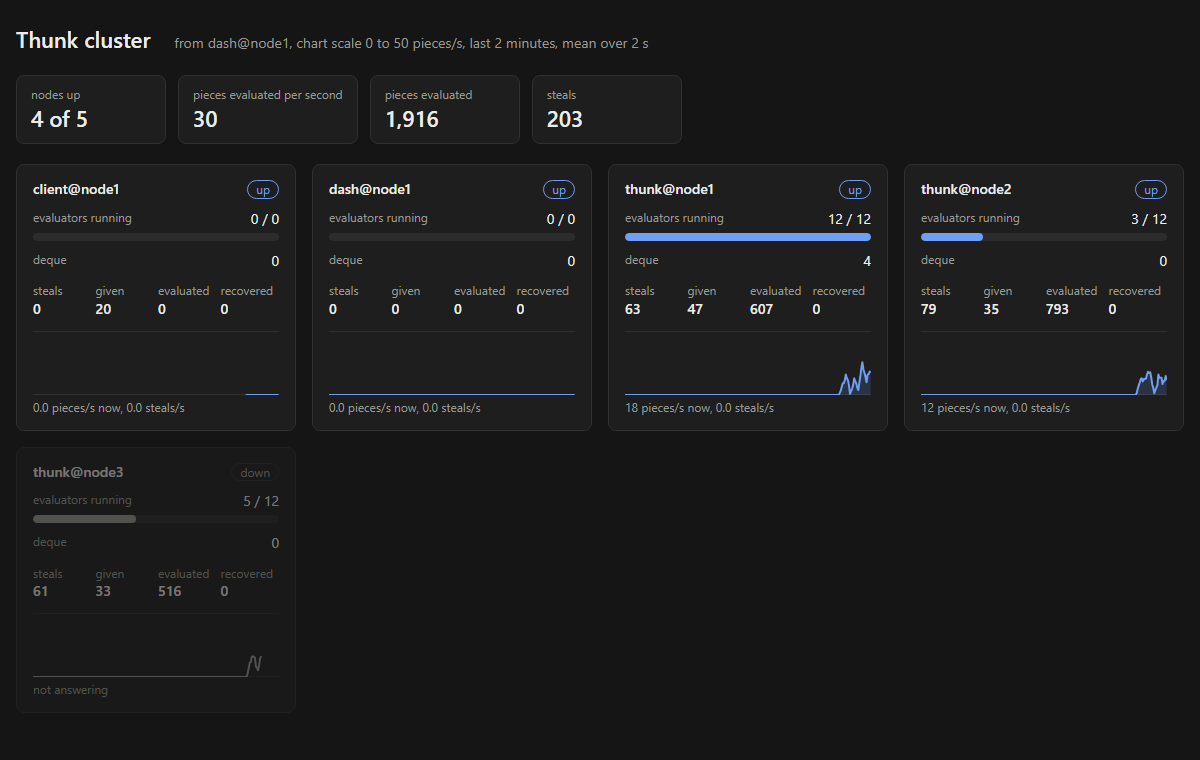
\includegraphics[width=0.65\textwidth]{figures/dashboard.png}
  \caption{The dashboard during the rendering of a $1280\times960$ image on the Compose cluster, a few seconds after \texttt{node3} was killed: the two surviving nodes are computing, the submitter and the dashboard node compute nothing, and the lost node stays on the page as down.}
  \label{fig:dashboard}
\end{figure}

\paragraph{Simulating node failures.}
While a long job is running, a node can be stopped from another terminal:
\begin{lstlisting}
docker compose kill node3
\end{lstlisting}
The job completes, and the \texttt{recovered} counters show which nodes recomputed the lost pieces.

\section{Self-evaluation}\label{self-evaluation}

This project was entirely designed and implemented as an individual effort by Yosberto Baro Carbonell.

\subsection{Strengths}

\begin{itemize}
  \item \textbf{Fully decentralized architecture:} no master, no central queue, no shared store; pieces are stolen between computing nodes, not only from the submitter.
  \item \textbf{Computations as data:} nodes do not need to know a program in advance, and no compiled code is ever exchanged.
  \item \textbf{Fault tolerance without replication:} node crashes are tolerated by recomputation, and results are always identical to a sequential reference.
  \item \textbf{Testing with real nodes:} automated tests start real additional nodes and stop them in the middle of jobs; the cluster is reproducible with Docker Compose.
\end{itemize}

\subsection{Weaknesses and Limitations}

\begin{itemize}
  \item \textbf{Small-scale evaluation:} most experiments ran on one laptop, and the multi-machine ones on two machines, one shared with other services; scaling beyond two machines has not been measured.
  \item \textbf{Lazy recovery:} the owner of a lost piece notices the loss only when it needs the result, which can be long after the node failed.
  \item \textbf{No tolerance of the submitting node's failure:} it holds the root of the job.
  \item \textbf{Closures carry their whole environment:} functions written inside other functions may carry unused data with every piece.
  \item \textbf{Interpretation cost:} much slower than native code, a deliberate trade-off that makes computations mobile and keeps the runtime independent of the programs.
  \item \textbf{No security:} the system assumes a trusted network; across the Internet it was protected by an SSH tunnel, not by the system itself.
\end{itemize}

\subsection{Overall Assessment}

The project achieves the objectives of the approved proposal, a combinator API with recursive decomposition, decentralized work stealing and a multi-node Docker Compose demonstration, and extends them with recovery from node failures, dynamic membership and a live dashboard.
%
Its main lesson is how the choice of the computation model removes problems that would otherwise need dedicated protocols: termination detection is unnecessary with fork-join, and consistency of results follows from purity.

\section{Future Works}\label{future-works}

\begin{itemize}
  \item \textbf{Larger evaluation:} more than two dedicated machines, to measure how the speed-up grows with the number of nodes and how the division of work depends on the network.
  \item \textbf{Proactive recovery:} a worker already knows which thief took each of its pieces; it could monitor thieves and put lost pieces back in its deque as soon as a node fails, instead of waiting for their owners to notice.
  \item \textbf{Capture of used variables only:} closures could capture only the variables their body uses, making every piece minimal; since this changes when two functions are equal, it is a decision about the language.
  \item \textbf{Improved stealing policies:} stealing half of a victim's deque, or choosing victims according to their load, are known refinements of randomized work stealing.
  \item \textbf{Membership at larger scale:} a larger cluster would need partial views, where each node knows only a sample of the others instead of all of them.
  \item \textbf{Parallel text processing:} splitting the text of the word count inside the parallel part of the job, to distribute tokenization too.
  \item \textbf{Native code generation:} translating programs into Erlang modules compiled and loaded at run time. Compiling closures into trees of Elixir functions was tried and was no faster than the interpreter.
  \item \textbf{Language extensions:} floating-point numbers, list literals, and error messages that point to the line of the source where a run-time error happened.
  \item \textbf{Security:} running the Erlang distribution over TLS, for clusters that cannot assume a trusted network.
  \item \textbf{Termination detection:} needed by an asynchronous task model, where no process waits for the pieces it creates, for example to reclaim the work of a job whose submitter failed.
\end{itemize}

{\small
\bibliographystyle{plain}
\bibliography{references}
}

\end{document}
